%!TeX root=../tese.tex
%("dica" para o editor de texto: este arquivo é parte de um documento maior)
% para saber mais: https://tex.stackexchange.com/q/78101/183146

%% ------------------------------------------------------------------------- %%
\chapter{Interpretação geométrica de buscas em ABBs}
\label{cap:geometria}

Neste capítulo iremos entender como interpretar de maneira geométrica os algoritmos de busca em ABBs.

\section{Visão geométrica de buscas}

Os algoritmos de busca dentro do modelo de computação adotado sempre iniciam o nó corrente na raiz da ABB e percorrem a árvore comparando a chave procurada com o nó corrente até encontrar o nó buscado.

Dada uma sequência $X = (x_{1},\ldots,x_{m})$ de $m$ acessos às chaves $x_{1}, x_{2},\ldots,x_{m}$, é possível ilustrar essa sequência $X$ de maneira gráfica em um plano cartesiano da seguinte forma: o eixo X representará as chaves armazenadas dentro da ABB e o eixo Y representará o tempo, ou seja, as buscas feitas nessa ABB. Assim, um ponto de coordenada ($x$,$y$) representa a busca da chave $x$ na ABB no instante de tempo $y$. Veja o exemplo da Figura~\ref{fig:geometria-inicial}.

\textit{Conjuntos arboreamente satisfeitos}: um par de pontos $(a,b)$ do conjunto $P$ é arboreamente satisfeito se $a$ e $b$ são ortogonalmente colineares ou se há pelo menos um ponto do conjunto \( P \setminus \{a,b\} \) que está dentro da área delimitada pelo retângulo de vértices $a$ e $b$. Um conjunto $P$ é arboreamente satisfeito se todos os pares de pontos do conjunto são arboreamente satisfeitos. Veja a Figura~\ref{fig:geometria-inicial}.

\begin{figure}[h!]
    \centering
    \begin{minipage}[b]{0.45\textwidth}
        \centering
        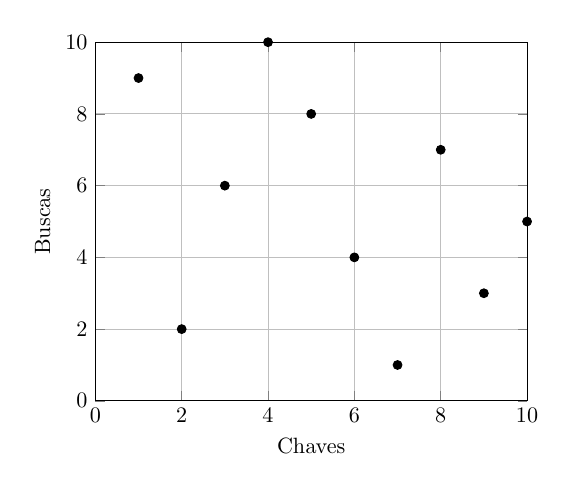
\begin{tikzpicture}[scale=0.8]
        \begin{axis}[
            xlabel={Chaves},
            ylabel={Buscas},
            grid=major,
            xmin=0, xmax=10,
            ymin=0, ymax=10,
            xtick={0,2,4,6,8,10},
            ytick={0,2,4,6,8,10}
        ]
        \addplot[only marks, mark=*] coordinates {
            (1,9)
            (2,2)
            (3,6)
            (4,10)
            (5,8)
            (6,4)
            (7,1)
            (8,7)
            (9,3)
            (10,5)
        };
        \end{axis}
        \end{tikzpicture}
    \end{minipage}\hfill
    \begin{minipage}[b]{0.45\textwidth}
        \centering
        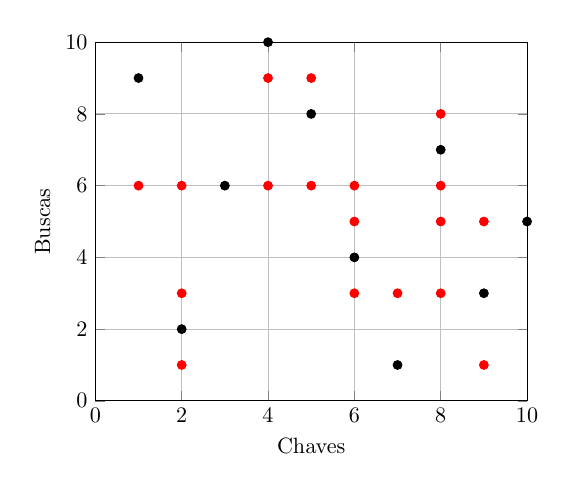
\begin{tikzpicture}[scale=0.8]
        \begin{axis}[
            xlabel={Chaves},
            ylabel={Buscas},
            grid=major,
            xmin=0, xmax=10,
            ymin=0, ymax=10,
            xtick={0,2,4,6,8,10},
            ytick={0,2,4,6,8,10}
        ]
        \addplot[only marks, mark=*] coordinates {
            (1,9)
            (2,2)
            (3,6)
            (4,10)
            (5,8)
            (6,4)
            (7,1)
            (8,7)
            (9,3)
            (10,5)
        };

        \addplot[only marks, mark=*, red] coordinates {
            (2,1)
            (9,1)
            (2,3)
            (6,3)
            (7,3)
            (8,3)
            (6,5)
            (8,5)
            (9,5)
            (1,6)
            (2,6)
            (4,6)
            (5,6)
            (6,6)
            (8,6)
            (8,8)
            (4,9)
            (5,9)
        };
        \end{axis}
        \end{tikzpicture}
    \end{minipage}
    \caption{À esquerda, um gráfico representando a busca (7, 2, 9, 6, 10, 3, 8, 5, 1, 4). À direita, um gráfico representando a mesma busca porém com um conjunto arboreamente satisfeito de pontos.}
\label{fig:geometria-inicial}
\end{figure}

%Em um conjunto arboreamente satisfeito, todo par de pontos $(a,b)$ não ortogonalmente colineares que não possuiem  
%menor conjunto de pontos sempre tem dois em linha ou nas pontas pelo menos

Em um conjunto arboreamento satisfeito, todo par de pontos $(a,b)$ não ortogonalmente colineares, há sempre pelo menos um ponto de \( P \setminus \{a,b\} \) que está em alguma aresta que incide em $a$, e há também pelo menos um ponto que está em alguma aresta que incide em $b$.

% falta caption
\begin{center}
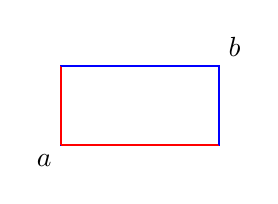
\begin{tikzpicture}
    \draw[blue, thick] (0,0) rectangle (2,1);
    
    \node at (0,0) [below left] {$a$};
    \node at (2,1) [above right] {$b$};
    
    \draw[red, thick] (0,0) -- (0,1);
    \draw[red, thick] (0,0) -- (2,0);
    \draw[blue, thick] (2,1) -- (0,1);
    \draw[blue, thick] (2,1) -- (2,0);
\end{tikzpicture}
\end{center}

\textbf{Prova:} Sejam $a$ e $b$ dois pontos de um conjunto arboreamente satisfeito. Como $(a,b)$ é um par de pontos arboreamente satisfeitos, então a área delimitada pelo retângulo de vértices $a$ e $b$ possui pelo menos 1 ponto diferente de $\{a,b\}$. Denotemos por $c$ tal ponto. Se $c$ não estiver em uma aresta que incide em $a$, então é possível recursivamente procurar tal ponto no par $(a,c)$ de pontos arboreamente satisfeitos. Analogamente, se $c$ não estiver em uma aresta que incide em $b$, então é possível recursivamente procurar tal ponto no par par $(c,b)$ de pontos arboreamente satisfeitos.

%Seja $\tau_i$ a subárvore // falar de subarvores?

A visão geométrica da execução de um algoritmo de busca em ABB para uma sequência $X = (x_{1},\ldots,x_{m})$ de buscas, de maneira similar, é o conjunto de pontos na forma ($x$,$y$) tal que $x$ foi uma chave acessada durante o instante de tempo $y$. É possível mapear esse conjunto de pontos para um plano cartesiano. Logo, todos os pontos com altura $y$ representam as chaves acessadas durante o instante de tempo $y$, ou seja, os nós acessados durante a busca por $x_y$. 
%não sei se eu gostei de $x_y$, porque $x$ é tanto coordenada quanto ponto na sequencia de busca

\textit{Lema 1.} A visão geométrica de qualquer execução de um algoritmo de busca em ABB no modelo de computação adotado é um conjunto de pontos arboreamente satisfeitos.

\textbf{Prova:} Assuma que a visão geométrica de um algoritmo de busca em ABB não é arboreamento satisfeita. Dessa maneira, há pelo menos um par de pontos $(a,b)$ nesse conjunto que não é arboreamente satisfeito. Seja $a$ a chave buscada no instante de tempo $i$ e seja $b$ a chave buscada no instante de tempo $j$. Assumiremos também sem perda de generalidade que $i < j$ e $a < b$.

Seja $c$ o ancestral comum mais profundo de $a$ e $b$ imediatamente antes da busca $i$. E seja $d$ o acestral comum mais profundo de $a$ e $b$ imediatamente antes da busca $j$.

Denotaremos números para áreas específicas para simplificar a explicação da prova. 
Área 1 = \{$(x,y)$ | $x = a$ e $i < y \leq j$\}, representando todos os acessos a $x$ entre os instantes de tempo $i$ e $j$. \\
Área 2 = \{$(x,y)$ | $a \leq x < b$ e $y = j$\}, representando todos os acessos a chaves entre $a$ e $b$ no instante de tempo $j$. \\
Área 3 = \{$(x,y)$ | $x = b$ e $i < y \leq j$\}, representando todos os acessos a $y$ entre os instantes de tempo $i$ e $j$. \\
Área 4 = \{$(x,y)$ | $a \leq x < b$ e $y = j$\}, representando todos os acessos a chaves entre $a$ e $b$ no instante de tempo $i$. \\
%Área 5 = \{$(x,y)$ | $a \leq x < b$ e $y = j$\}, representando todos os acessos a chaves entre $a$ e $b$ no instante de tempo $i$. \\

Como $(a,b)$ não são arboreamente satisfeitos, nota-se que não há nenhum ponto tanto nas bordas quanto no interior do retângulo de vértices $a$ e $b$. Logo $1 \cup 2 \cup 3 \cup 4 = \emptyset$.

\begin{figure}[H]
    \centering
    \begin{minipage}[t]{0.70\textwidth}
        Se $2 = \emptyset$, então $d = y$. Porém, se $d = y$ então, pelo menos em algum outro instante de tempo $h$, $h < j$, $y$ também era o ancestral comum mais profundo entre $a$ e $b$, logo $3 \neq \emptyset$. Por contrapositiva, se $3 = \emptyset \Rightarrow 2 \neq \emptyset$.

        Por $c$ ser o ancestral comum mais profundo de $a$ e $b$ no instante $i$, sabemos que $x \leq c \leq y$ e mais importante, $c$ está mais acima na ABB. Logo, para acessar qualquer chave no intervalo $[a,b]$, no instante $i$, é preciso acessar a chave $c$.
        
        Se $4 = \emptyset$, então $c = x$. Porém $b$ é acessado no instante $j$. Se $c = d$, $a$ precisa ser acessados no instante de tempo $j$, logo $1 \neq \emptyset$. Caso $c \neq d$, então em algum instante de tempo $h$, $i \leq h < j$, o ancestral comum mais profundo entre $a$ e $b$ mudou, logo algum nó com chave no intervalo $(a,b]$ precisa ter sido rotacionado para cima, porém de acordo com o modelo de computação só é possível rotacionar um nó depois de acessa-lo e sabemos que qualquer acesso no intervalo $[a,b]$ no instante de tempo $h$, precisa acessar o ancestral comum mais profundo que neste caso é $x$. Logo $1 \neq \emptyset$. Por contrapositiva, $1 = \emptyset \Rightarrow 4 \neq \emptyset$.

    \end{minipage}\hfill
    \begin{minipage}[t]{0.25\textwidth}
        % Coluna da direita com a imagem
        \centering
        \begin{adjustbox}{valign=t} % Alinha o gráfico ao topo da caixa
        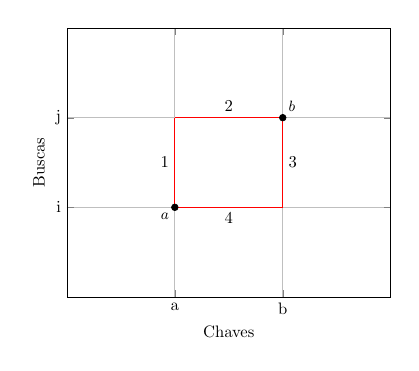
\begin{tikzpicture}[scale=0.6]
        \begin{axis}[
            xlabel={Chaves},
            ylabel={Buscas},
            grid=major,
            xmin=0, xmax=3,
            ymin=0, ymax=3,
            xtick={1,2},
            ytick={1,2},
            xticklabels={a,b}, % Define os rótulos do eixo x
            yticklabels={i,j} % Define os rótulos do eixo y
        ]

        \addplot[only marks, mark=*] coordinates {
            (1,1)
            (2,2)
        };

        \addplot[red, thick] coordinates {
            (1,2)
            (2,2)
        };

        \addplot[red, thick] coordinates {
            (2,2)
            (2,1)
        };

        \addplot[red, thick] coordinates {
            (1,1)
            (1,2)
        };

        \addplot[red, thick] coordinates {
            (1,1)
            (2,1)
        };

        % Adiciona rótulos aos pontos
        \node at (axis cs:1,1) [anchor=north east, fill=white, font=\small] {$a$};
        \node at (axis cs:2,2) [anchor=south west, fill=white, font=\small] {$b$};

        \node at (axis cs:1,1.5) [anchor=east, font=\normalsize] {1};
        \node at (axis cs:1.5,2) [anchor=south, font=\normalsize] {2};
        \node at (axis cs:2,1.5) [anchor=west, font=\normalsize] {3};
        \node at (axis cs:1.5,1) [anchor=north, font=\normalsize] {4};
        %\node at (axis cs:1.5,1.5) [anchor=center, font=\normalsize] {5};

        \end{axis}
        \end{tikzpicture}
        \end{adjustbox}
    \end{minipage}
    %\caption{Gráfico de chaves e buscas}
    \label{fig:chaves-buscas}
\end{figure}

Lema 2. Qualquer conjunto de pontos arboreamente satisfeitos representa a execução de um algoritmo de busca em ABB no modelo de computação adotado.